% Options for packages loaded elsewhere
\PassOptionsToPackage{unicode}{hyperref}
\PassOptionsToPackage{hyphens}{url}
\PassOptionsToPackage{dvipsnames,svgnames,x11names}{xcolor}
%
\documentclass[
  11pt,
  letterpaper,
  twoside]{report}

\usepackage{amsmath,amssymb}
\usepackage{setspace}
\usepackage{iftex}
\ifPDFTeX
  \usepackage[T1]{fontenc}
  \usepackage[utf8]{inputenc}
  \usepackage{textcomp} % provide euro and other symbols
\else % if luatex or xetex
  \usepackage{unicode-math}
  \defaultfontfeatures{Scale=MatchLowercase}
  \defaultfontfeatures[\rmfamily]{Ligatures=TeX,Scale=1}
\fi
\usepackage{lmodern}
\ifPDFTeX\else  
    % xetex/luatex font selection
\fi
% Use upquote if available, for straight quotes in verbatim environments
\IfFileExists{upquote.sty}{\usepackage{upquote}}{}
\IfFileExists{microtype.sty}{% use microtype if available
  \usepackage[]{microtype}
  \UseMicrotypeSet[protrusion]{basicmath} % disable protrusion for tt fonts
}{}
\makeatletter
\@ifundefined{KOMAClassName}{% if non-KOMA class
  \IfFileExists{parskip.sty}{%
    \usepackage{parskip}
  }{% else
    \setlength{\parindent}{0pt}
    \setlength{\parskip}{6pt plus 2pt minus 1pt}}
}{% if KOMA class
  \KOMAoptions{parskip=half}}
\makeatother
\usepackage{xcolor}
\usepackage[inner=1.5in,outer=1in,top=1in,bottom=1in,heightrounded]{geometry}
\setlength{\emergencystretch}{3em} % prevent overfull lines
\setcounter{secnumdepth}{2}

\usepackage{color}
\usepackage{fancyvrb}
\newcommand{\VerbBar}{|}
\newcommand{\VERB}{\Verb[commandchars=\\\{\}]}
\DefineVerbatimEnvironment{Highlighting}{Verbatim}{commandchars=\\\{\}}
% Add ',fontsize=\small' for more characters per line
\newenvironment{Shaded}{}{}
\newcommand{\AlertTok}[1]{\textcolor[rgb]{0.58,0.85,0.30}{\textbf{\colorbox[rgb]{0.30,0.12,0.14}{#1}}}}
\newcommand{\AnnotationTok}[1]{\textcolor[rgb]{0.31,0.63,0.31}{#1}}
\newcommand{\AttributeTok}[1]{\textcolor[rgb]{0.65,0.15,0.64}{#1}}
\newcommand{\BaseNTok}[1]{\textcolor[rgb]{0.60,0.41,0.00}{#1}}
\newcommand{\BuiltInTok}[1]{\textcolor[rgb]{0.65,0.15,0.64}{#1}}
\newcommand{\CharTok}[1]{\textcolor[rgb]{0.31,0.63,0.31}{#1}}
\newcommand{\CommentTok}[1]{\textcolor[rgb]{0.63,0.63,0.65}{\textit{#1}}}
\newcommand{\CommentVarTok}[1]{\textcolor[rgb]{0.89,0.34,0.29}{\textit{#1}}}
\newcommand{\ConstantTok}[1]{\textcolor[rgb]{0.60,0.41,0.00}{#1}}
\newcommand{\ControlFlowTok}[1]{\textcolor[rgb]{0.65,0.15,0.64}{#1}}
\newcommand{\DataTypeTok}[1]{\textcolor[rgb]{0.65,0.15,0.64}{#1}}
\newcommand{\DecValTok}[1]{\textcolor[rgb]{0.60,0.41,0.00}{#1}}
\newcommand{\DocumentationTok}[1]{\textcolor[rgb]{0.89,0.34,0.29}{#1}}
\newcommand{\ErrorTok}[1]{\textcolor[rgb]{0.96,0.28,0.28}{\underline{#1}}}
\newcommand{\ExtensionTok}[1]{\textcolor[rgb]{0.25,0.47,0.95}{\textbf{#1}}}
\newcommand{\FloatTok}[1]{\textcolor[rgb]{0.60,0.41,0.00}{#1}}
\newcommand{\FunctionTok}[1]{\textcolor[rgb]{0.25,0.47,0.95}{#1}}
\newcommand{\ImportTok}[1]{\textcolor[rgb]{0.31,0.63,0.31}{#1}}
\newcommand{\InformationTok}[1]{\textcolor[rgb]{0.77,0.36,0.00}{#1}}
\newcommand{\KeywordTok}[1]{\textcolor[rgb]{0.65,0.15,0.64}{#1}}
\newcommand{\NormalTok}[1]{\textcolor[rgb]{0.22,0.23,0.26}{#1}}
\newcommand{\OperatorTok}[1]{\textcolor[rgb]{0.65,0.15,0.64}{#1}}
\newcommand{\OtherTok}[1]{\textcolor[rgb]{0.15,0.68,0.38}{#1}}
\newcommand{\PreprocessorTok}[1]{\textcolor[rgb]{0.65,0.15,0.64}{#1}}
\newcommand{\RegionMarkerTok}[1]{\textcolor[rgb]{0.16,0.50,0.73}{\colorbox[rgb]{0.08,0.19,0.26}{#1}}}
\newcommand{\SpecialCharTok}[1]{\textcolor[rgb]{0.00,0.52,0.74}{#1}}
\newcommand{\SpecialStringTok}[1]{\textcolor[rgb]{0.85,0.27,0.33}{#1}}
\newcommand{\StringTok}[1]{\textcolor[rgb]{0.31,0.63,0.31}{#1}}
\newcommand{\VariableTok}[1]{\textcolor[rgb]{0.89,0.34,0.29}{#1}}
\newcommand{\VerbatimStringTok}[1]{\textcolor[rgb]{0.85,0.27,0.33}{#1}}
\newcommand{\WarningTok}[1]{\textcolor[rgb]{0.85,0.27,0.33}{#1}}

\providecommand{\tightlist}{%
  \setlength{\itemsep}{0pt}\setlength{\parskip}{0pt}}\usepackage{longtable,booktabs,array}
\usepackage{calc} % for calculating minipage widths
% Correct order of tables after \paragraph or \subparagraph
\usepackage{etoolbox}
\makeatletter
\patchcmd\longtable{\par}{\if@noskipsec\mbox{}\fi\par}{}{}
\makeatother
% Allow footnotes in longtable head/foot
\IfFileExists{footnotehyper.sty}{\usepackage{footnotehyper}}{\usepackage{footnote}}
\makesavenoteenv{longtable}
\usepackage{graphicx}
\makeatletter
\def\maxwidth{\ifdim\Gin@nat@width>\linewidth\linewidth\else\Gin@nat@width\fi}
\def\maxheight{\ifdim\Gin@nat@height>\textheight\textheight\else\Gin@nat@height\fi}
\makeatother
% Scale images if necessary, so that they will not overflow the page
% margins by default, and it is still possible to overwrite the defaults
% using explicit options in \includegraphics[width, height, ...]{}
\setkeys{Gin}{width=\maxwidth,height=\maxheight,keepaspectratio}
% Set default figure placement to htbp
\makeatletter
\def\fps@figure{htbp}
\makeatother
% definitions for citeproc citations
\NewDocumentCommand\citeproctext{}{}
\NewDocumentCommand\citeproc{mm}{%
  \begingroup\def\citeproctext{#2}\cite{#1}\endgroup}
\makeatletter
 % allow citations to break across lines
 \let\@cite@ofmt\@firstofone
 % avoid brackets around text for \cite:
 \def\@biblabel#1{}
 \def\@cite#1#2{{#1\if@tempswa , #2\fi}}
\makeatother
\newlength{\cslhangindent}
\setlength{\cslhangindent}{1.5em}
\newlength{\csllabelwidth}
\setlength{\csllabelwidth}{3em}
\newenvironment{CSLReferences}[2] % #1 hanging-indent, #2 entry-spacing
 {\begin{list}{}{%
  \setlength{\itemindent}{0pt}
  \setlength{\leftmargin}{0pt}
  \setlength{\parsep}{0pt}
  % turn on hanging indent if param 1 is 1
  \ifodd #1
   \setlength{\leftmargin}{\cslhangindent}
   \setlength{\itemindent}{-1\cslhangindent}
  \fi
  % set entry spacing
  \setlength{\itemsep}{#2\baselineskip}}}
 {\end{list}}
\usepackage{calc}
\newcommand{\CSLBlock}[1]{\hfill\break\parbox[t]{\linewidth}{\strut\ignorespaces#1\strut}}
\newcommand{\CSLLeftMargin}[1]{\parbox[t]{\csllabelwidth}{\strut#1\strut}}
\newcommand{\CSLRightInline}[1]{\parbox[t]{\linewidth - \csllabelwidth}{\strut#1\strut}}
\newcommand{\CSLIndent}[1]{\hspace{\cslhangindent}#1}

\usepackage{booktabs}
\usepackage{caption}
\usepackage{longtable}
\makeatletter
\@ifpackageloaded{tcolorbox}{}{\usepackage[skins,breakable]{tcolorbox}}
\@ifpackageloaded{fontawesome5}{}{\usepackage{fontawesome5}}
\definecolor{quarto-callout-color}{HTML}{909090}
\definecolor{quarto-callout-note-color}{HTML}{0758E5}
\definecolor{quarto-callout-important-color}{HTML}{CC1914}
\definecolor{quarto-callout-warning-color}{HTML}{EB9113}
\definecolor{quarto-callout-tip-color}{HTML}{00A047}
\definecolor{quarto-callout-caution-color}{HTML}{FC5300}
\definecolor{quarto-callout-color-frame}{HTML}{acacac}
\definecolor{quarto-callout-note-color-frame}{HTML}{4582ec}
\definecolor{quarto-callout-important-color-frame}{HTML}{d9534f}
\definecolor{quarto-callout-warning-color-frame}{HTML}{f0ad4e}
\definecolor{quarto-callout-tip-color-frame}{HTML}{02b875}
\definecolor{quarto-callout-caution-color-frame}{HTML}{fd7e14}
\makeatother
\makeatletter
\@ifpackageloaded{bookmark}{}{\usepackage{bookmark}}
\makeatother
\makeatletter
\@ifpackageloaded{caption}{}{\usepackage{caption}}
\AtBeginDocument{%
\ifdefined\contentsname
  \renewcommand*\contentsname{Table of contents}
\else
  \newcommand\contentsname{Table of contents}
\fi
\ifdefined\listfigurename
  \renewcommand*\listfigurename{List of Figures}
\else
  \newcommand\listfigurename{List of Figures}
\fi
\ifdefined\listtablename
  \renewcommand*\listtablename{List of Tables}
\else
  \newcommand\listtablename{List of Tables}
\fi
\ifdefined\figurename
  \renewcommand*\figurename{Figure}
\else
  \newcommand\figurename{Figure}
\fi
\ifdefined\tablename
  \renewcommand*\tablename{Table}
\else
  \newcommand\tablename{Table}
\fi
}
\@ifpackageloaded{float}{}{\usepackage{float}}
\floatstyle{ruled}
\@ifundefined{c@chapter}{\newfloat{codelisting}{h}{lop}}{\newfloat{codelisting}{h}{lop}[chapter]}
\floatname{codelisting}{Listing}
\newcommand*\listoflistings{\listof{codelisting}{List of Listings}}
\makeatother
\makeatletter
\makeatother
\makeatletter
\@ifpackageloaded{caption}{}{\usepackage{caption}}
\@ifpackageloaded{subcaption}{}{\usepackage{subcaption}}
\makeatother
\makeatletter
\@ifpackageloaded{tcolorbox}{}{\usepackage[skins,breakable]{tcolorbox}}
\makeatother
\makeatletter
\@ifundefined{shadecolor}{\definecolor{shadecolor}{rgb}{.97, .97, .97}}{}
\makeatother
\makeatletter
\@ifundefined{codebgcolor}{\definecolor{codebgcolor}{HTML}{f8f8f8}}{}
\makeatother
\makeatletter
\ifdefined\Shaded\renewenvironment{Shaded}{\begin{tcolorbox}[enhanced, borderline west={3pt}{0pt}{shadecolor}, sharp corners, colback={codebgcolor}, frame hidden, boxrule=0pt, breakable]}{\end{tcolorbox}}\fi
\makeatother

\ifLuaTeX
  \usepackage{selnolig}  % disable illegal ligatures
\fi
\usepackage{bookmark}

\IfFileExists{xurl.sty}{\usepackage{xurl}}{} % add URL line breaks if available
\urlstyle{same} % disable monospaced font for URLs
\hypersetup{
  pdftitle={Parallel Computation Framework for Discrete Copula Modeling},
  pdfauthor={Dhyey Mavani},
  colorlinks=true,
  linkcolor={blue},
  filecolor={Maroon},
  citecolor={Blue},
  urlcolor={Blue},
  pdfcreator={LaTeX via pandoc}}

% Custom fonts
% See https://ctan.math.utah.edu/ctan/tex-archive/fonts/xcharter/doc/xcharter-doc.pdf

\usepackage[sups]{XCharter}% lining figures in math
\usepackage[scaled=1.04,varqu,varl]{inconsolata}% inconsolata typewriter
\usepackage[type1]{sourcesanspro}% sans serif
\usepackage[uprightscript,charter,vvarbb,scaled=1.05]{newtxmath}
%% See Amherst College Thesis Guide
%% https://www.amherst.edu/academiclife/registrar/for-students/thesis_guide
% For Interdisciplinary majors, the statement should read "Submitted to the Department of Special Programs of Amherst College in partial fulfillment of the requirements for the degree of Bachelor of Arts with honors." 
% For those students submitting a thesis in either Greek or Latin, please print the statement in the following manner: "Submitted to the Department of Classics of Amherst College in partial fulfillment of the requirements for the degree of Bachelor of Arts with honors in Greek/Latin."
\def\maketitle{
\pagenumbering{roman}
{\thispagestyle{empty}%
  \null\vskip 1in
  \begin{center}\fontsize{24}{28}\sf
     \textbf{Parallel Computation Framework for Discrete Copula
Modeling}\\[2cm]
     \fontsize{18}{20}\sf Dhyey Mavani\\[0.2cm]
     
     \vfill
     
     
\includegraphics[height=1.15in]{includes/Amherst-College-wordmark-seal-centered-purple-RGB-900px.png}
     \vskip 0.5in
     \fontsize{13}{15}\sf Submitted to the Department of Mathematics and
Statistics\\
     of Amherst College in partial fulfillment of the requirements \\
     for the degree of Bachelor of Arts with honors.\\
     \vskip 0.5in
     Advisor(s):\\
     \fontsize{13}{15}\sf Professor Shu-Min Liao
    \vskip 0.5in
    October 15, 2024
  \end{center}
  \newpage\mbox{}\thispagestyle{empty}\newpage
}
}

% Title and date

\title{Parallel Computation Framework for Discrete Copula Modeling}

\begin{document}
\maketitle

\renewcommand*\contentsname{Table of contents}
{
\hypersetup{linkcolor=}
\setcounter{tocdepth}{1}
\tableofcontents
}

\setstretch{2}
\bookmarksetup{startatroot}

\chapter*{Abstract}\label{abstract}
\addcontentsline{toc}{chapter}{Abstract}

\markboth{Abstract}{Abstract}

Categorical data, particularly when involving ordinal responses, plays a
crucial role in fields such as social sciences and finance, where
capturing the inherent ordering of variables can lead to more meaningful
inferences of the underlying distributions. A key challenge in analyzing
such data lies in exploring the regression dependence structures among
variables. While many model-based approaches have been developed to
examine these structures, there remains a scarcity of model-free
methods. Wei \& Kim (2021) addressed this gap by introducing SCCRAM, a
novel model-free measure based on the checkerboard copula, capable of
identifying and quantifying regression dependence in multivariate
categorical data with ordinal and nominal variables. This work builds on
their contribution by developing scalable R and Python packages for
SCCRAM, employing parallel computing to enhance accessibility and
efficiency in large-scale data analysis. Initial simulations demonstrate
the effectiveness of these implementations, offering researchers a
robust tool for exploratory modeling and further exploration of
regression dependence structures in categorical datasets for this
use-case.

\bookmarksetup{startatroot}

\chapter*{Acknowledgements}\label{acknowledgements}
\addcontentsline{toc}{chapter}{Acknowledgements}

\markboth{Acknowledgements}{Acknowledgements}

I would like to thank everyone who made my experience nothing short of
amazing during my thesis journey. Firstly, I'd like to convey my
gratitude to Professor Shu-Min Liao for advising me through this
journey, and for believing in me to take on statistical software
component of her most recent research work along with her collaborators.
From my first research experience on campus building R-Blocks, she
played a pivotal role in my journey.

I am also incredibly grateful to my college advisor, and statistics
major advisor, Professor Nicholas Horton for always advocating for me
and for supporting me throughout the Amherst College experience. I would
also like to thank Professor Jun Ishii for teaching me Advanced
Econometrics, which helped me gain a really clear understanding on the
foundational tools on which I was able to build on in my work.

Finally, I would like to thank my friends and family for their constant
belief in my abilities. Special thanks to my mom, dad, sister,
grandfather, and grandmother for lending me and making me capable for
this opportunity to study abroad. Last, but not the least, I would like
to thank my friends, peers, and colleagues on campus, who took courses,
worked, and played sports with me. This journey of academic, personal,
and professional growth wouldn't be possible without their support.

\cleardoublepage\pagenumbering{arabic}\setcounter{page}{1}

\bookmarksetup{startatroot}

\chapter{Intro to your Quarto Book thesis}\label{sec-intro}

This template uses a Quarto Book project to generate your thesis
document. This document includes important information about how to
navigate this project directory and use the Quarto Book project.

To use the
\href{https://github.com/Amherst-Statistics/thesis?tab=readme-ov-file\#amherst-college-statistics-thesis-template}{Amherst
College Statistics Thesis Template}, do \textbf{one} of the following:

\begin{itemize}
\item
  Download the repo.
\item
  Fork the repo.
\item
  Using the command line or terminal, go to the directory where you want
  your thesis project directory to be stored and run the following to
  copy the contents of the repo:

\begin{Shaded}
\begin{Highlighting}[numbers=left,,]
\NormalTok{quarto use template Amherst{-}Statistics/thesis}
\end{Highlighting}
\end{Shaded}
\end{itemize}

\section{What's in this project
directory?}\label{whats-in-this-project-directory}

\begin{itemize}
\item
  \texttt{\_extensions} folder: contains additional files for formatting
  the thesis. Do not delete, edit, or move this folder or its contents.
\item
  \texttt{\_quarto.yml} file. Do not rename, move, or delete this file.

  \begin{itemize}
  \tightlist
  \item
    This file controls the structure and formatting of your thesis.
  \item
    Update this file with your thesis information, the list of qmd files
    to include when rendering the document, and the name of your
    bibliography file.
  \end{itemize}
\item
  \texttt{.qmd} files containing the contents of your thesis.

  \begin{itemize}
  \tightlist
  \item
    You should \textbf{not} delete or rename the \texttt{index.qmd}
    file. It must be included as named the first rendered file of your
    thesis. This file includes your acknowledgements, abstract, and a
    reproducibility statement. Be sure to edit these sections before
    your final thesis submission!
  \item
    You should \textbf{not} delete the
    \hyperref[references]{\emph{references}} or the \emph{appendix}
    files (Appendix~\ref{sec-code}, Appendix~\ref{sec-corrections})
    which contain syntax and information required for proper thesis
    formatting, but you can and should rename them as needed.
  \item
    You should delete the \emph{chapter} files and replace them with
    your own.
  \end{itemize}
\item
  \texttt{includes} folder: contains citation style file (for formatting
  in-text citations and the bibliography using the ASA style) and the
  Amherst logo included on the cover page. Do not delete, edit, or move
  this folder or its contents.
\item
  \texttt{data} folder: recommended folder for storing data files
\item
  \texttt{fig} folder: recommended folder for storing any images,
  graphs, etc.
\item
  \texttt{src} folder: recommended folder for storing any code scripts.
\end{itemize}

\begin{tcolorbox}[enhanced jigsaw, coltitle=black, leftrule=.75mm, rightrule=.15mm, breakable, titlerule=0mm, bottomrule=.15mm, left=2mm, colbacktitle=quarto-callout-note-color!10!white, arc=.35mm, toprule=.15mm, title=\textcolor{quarto-callout-note-color}{\faInfo}\hspace{0.5em}{Note}, toptitle=1mm, colback=white, bottomtitle=1mm, opacitybacktitle=0.6, opacityback=0, colframe=quarto-callout-note-color-frame]

Items in the \texttt{data}, \texttt{fig}, and \texttt{src} folders
starting with \texttt{temp} are used as examples within this template
but can be deleted when you begin your own edits.

\end{tcolorbox}

\begin{itemize}
\item
  After rendering your document, you will additionally see a
  \texttt{\_book} folder, which will contain the rendered PDF.
\item
  \texttt{references.bib}: This is a bibliography file containing
  bibtex-style citation information. BibTeX is a format for citations
  used by LaTeX, which is the language that is used in the process of
  rendering the document to PDF. The format uses \emph{citation keys},
  which are unique identifiers for each citation that you can customize
  manually or through the use of citation management software. These
  citation keys are what are used to make in-text cross-references
  throughout your thesis.

  \begin{itemize}
  \tightlist
  \item
    You can rename the \texttt{.bib} file, just make sure to update the
    filename in the \texttt{\_quarto.yml} file.
  \item
    Consider using \href{https://www.zotero.org/support/}{Zotero} for
    managing all of the literature affiliated with your thesis. Amherst
    College has
    \href{https://libguides.amherst.edu/citation/zotero}{Zotero support
    and free unlimited storage} through the library.
  \item
    You can
    \href{https://libguides.rhul.ac.uk/referencing/Zoterolatex}{set up
    Zotero to automatically update your \texttt{.bib} file} that
    contains all of your reference information.
    \href{https://guides.library.yale.edu/bibtex/zotero-and-latex}{Video
    setup instructions are also available}.
  \item
    \href{https://libguides.amherst.edu/subjectlibrarians\#s-lg-box-31290705}{Set
    up an appointment with a science librarian} at Amherst or attend one
    of the library's
    \href{https://libguides.amherst.edu/c.php?g=959622&p=6928473\#s-lg-box-22237086}{Zotero
    workshops} to learn more. Your thesis advisor should also be able to
    help.
  \end{itemize}
\end{itemize}

\section{Quarto workflow}\label{quarto-workflow}

\begin{enumerate}
\def\labelenumi{\arabic{enumi}.}
\item
  Create and edit \texttt{.qmd} files.

  \begin{itemize}
  \tightlist
  \item
    When naming chapter and appendix files, we recommend leading the
    filename with the number of its rendering order.
  \item
    The \texttt{index.qmd} file must remain named \texttt{index.qmd}
  \end{itemize}
\item
  Update the \texttt{\_quarto.yml} file.

  \begin{itemize}
  \tightlist
  \item
    Add or remove \texttt{.qmd} files to the list of \texttt{chapters}
    or \texttt{appendices} as appropriate. You can also temporarily
    comment out chapters.
  \item
    Save your own \texttt{.bib} file and make sure the filename is
    updated in \texttt{\_quarto.yml}.
  \end{itemize}
\item
  Render book

  \begin{itemize}
  \tightlist
  \item
    Type \texttt{cmd\ +\ shift\ +\ k} or \texttt{ctrl\ +\ shift\ +\ k}
    while working in any of your \texttt{.qmd} files, use the
    \texttt{Render} button at the top of any \texttt{.qmd} file, or use
    the \texttt{Render} button available under the \texttt{Build} tab.
  \item
    If you would like the PDF to preview within the RStudio Viewer pane,
    click the gear icon next to the \texttt{Render} button at the top of
    any of your \texttt{.qmd} files and select \textbf{Preview in Viewer
    Pane.} It will change the default behavior until you make a
    different selection.
  \end{itemize}

  \begin{center}
  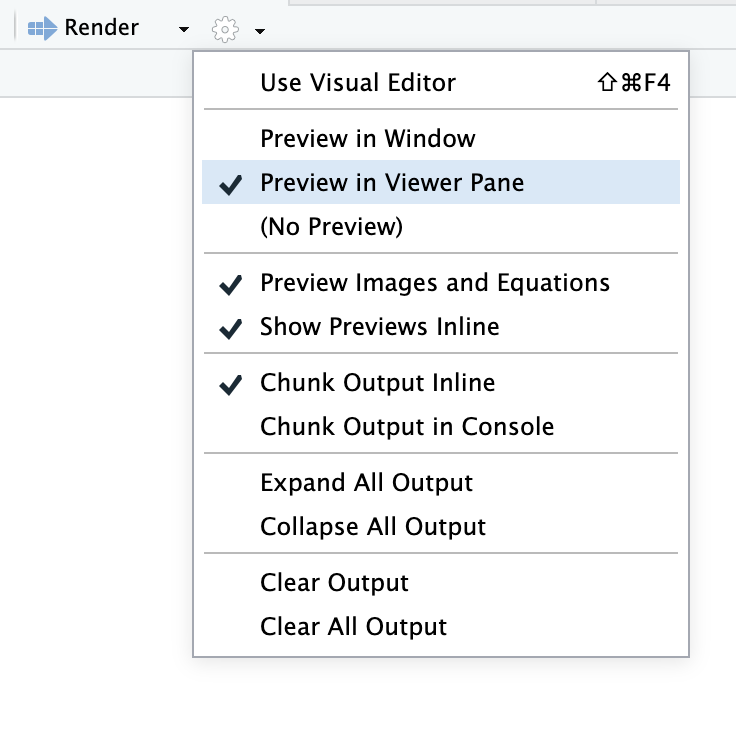
\includegraphics[width=0.5\textwidth,height=\textheight]{fig/temp_preview-viewer-pane.png}
  \end{center}

  \begin{tcolorbox}[enhanced jigsaw, coltitle=black, leftrule=.75mm, rightrule=.15mm, breakable, titlerule=0mm, bottomrule=.15mm, left=2mm, colbacktitle=quarto-callout-note-color!10!white, arc=.35mm, toprule=.15mm, title=\textcolor{quarto-callout-note-color}{\faInfo}\hspace{0.5em}{Note}, toptitle=1mm, colback=white, bottomtitle=1mm, opacitybacktitle=0.6, opacityback=0, colframe=quarto-callout-note-color-frame]

  Rendering any \texttt{.qmd} file will render the \emph{entire} project
  (all files listed under \texttt{chapters} in the
  \texttt{\_quarto.yml}).

  If you want to focus on one particular chapter without running code in
  or rendering other chapters, delete or comment out the other chapter
  files in \texttt{\_quarto.yml}. The \texttt{index.qmd} file must
  always be included in the rendering list, though.

  \end{tcolorbox}
\item
  Review the changes in the PDF (located in the \texttt{\_book} folder)
  to ensure the PDF output looks as desired. Here are some common issues
  you might want to look for:

  \begin{itemize}
  \item
    No text, figures, tables, nor code extends into the margins
  \item
    Citations and cross-references are displayed correctly and linked
    correctly
  \item
    Font in figures and tables is readable
  \item
    All
    \href{https://quarto.org/docs/authoring/cross-references.html\#floats}{figures
    and tables} are captioned and numbered
  \item
    Any
    \href{https://quarto.org/docs/authoring/cross-references.html\#equations}{equations}
    that are referenced in the text should also be numbered.
  \item
    Make appropriate use of Quarto's
    \href{https://quarto.org/docs/authoring/cross-references.html\#theorems-and-proofs}{theorem
    and proof} blocks when needed.
  \item
    Though
    \href{https://quarto.org/docs/authoring/callouts.html}{callout
    blocks} might be useful for inserting notes to yourself or your
    advisor, they are likely not appropriate for your final thesis and
    should be excluded.
  \item
    Figures are visually appealing (aspect ratio, appropriate use of
    aesthetics for contrast, etc.)
  \item
    Headings, subheadings, lists, sublists, etc. are formatted
    correctly. Errors are usually due to indentation or line spacing
    before headings or lists.

    \begin{tcolorbox}[enhanced jigsaw, coltitle=black, leftrule=.75mm, rightrule=.15mm, breakable, titlerule=0mm, bottomrule=.15mm, left=2mm, colbacktitle=quarto-callout-note-color!10!white, arc=.35mm, toprule=.15mm, title=\textcolor{quarto-callout-note-color}{\faInfo}\hspace{0.5em}{Note}, toptitle=1mm, colback=white, bottomtitle=1mm, opacitybacktitle=0.6, opacityback=0, colframe=quarto-callout-note-color-frame]

    To format additional content within a list item at the same depth,
    the first text of the new content must align with the first text of
    the corresponding list item text above it. For example, the first
    colon \texttt{:} of this callout block is aligned with the first
    letter of the bullet point above.

    \end{tcolorbox}
  \end{itemize}

  \emph{In comparison, this text will be indented to the same depth as
  the text in item 4.}
\end{enumerate}

\section{Recommended reading before you begin
editing}\label{recommended-reading-before-you-begin-editing}

Quarto is a powerful tool for authoring documents in multiple formats.
Even if you are familiar with markdown, some behavior and syntax in
Quarto markdown is slightly different (and often better) than R
markdown.

\begin{tcolorbox}[enhanced jigsaw, coltitle=black, leftrule=.75mm, rightrule=.15mm, breakable, titlerule=0mm, bottomrule=.15mm, left=2mm, colbacktitle=quarto-callout-caution-color!10!white, arc=.35mm, toprule=.15mm, title=\textcolor{quarto-callout-caution-color}{\faFire}\hspace{0.5em}{Caution}, toptitle=1mm, colback=white, bottomtitle=1mm, opacitybacktitle=0.6, opacityback=0, colframe=quarto-callout-caution-color-frame]

The code within each \texttt{.qmd} file is self-contained and rendered
independently before merging the document to build the thesis, so
there's no environmental memory between chapters. This means you should
load required packages and datasets and set up any desired code defaults
at the start of each chapter file.

\end{tcolorbox}

\begin{enumerate}
\def\labelenumi{\arabic{enumi}.}
\item
  \href{https://quarto.org/docs/authoring/markdown-basics.html}{Quarto
  Markdown Basics}, how to
  \href{https://quarto.org/docs/computations/inline-code.html}{use
  inline code} with the Knitr engine, and more details on
  \href{https://quarto.org/docs/authoring/figures.html}{including
  external figures}.

  \begin{tcolorbox}[enhanced jigsaw, coltitle=black, leftrule=.75mm, rightrule=.15mm, breakable, titlerule=0mm, bottomrule=.15mm, left=2mm, colbacktitle=quarto-callout-note-color!10!white, arc=.35mm, toprule=.15mm, title=\textcolor{quarto-callout-note-color}{\faInfo}\hspace{0.5em}{Note}, toptitle=1mm, colback=white, bottomtitle=1mm, opacitybacktitle=0.6, opacityback=0, colframe=quarto-callout-note-color-frame]

  Many options will work for both PDF and HTML formats, but your thesis
  must be submitted as a PDF. Pay attention to which elements work for
  both formats and which elements are only appropriate for HTML format.
  You need to prioritize the PDF rendering.

  \end{tcolorbox}
\item
  \href{https://quarto.org/docs/computations/r.html\#chunk-options}{How
  to specify code chunk options in Quarto} and the
  \href{https://quarto.org/docs/computations/execution-options.html}{list
  of code chunk options} (the Quarto Book is rendered using the KnitR
  engine so you can follow links on the latter page to see additional
  options). The document-level defaults set \texttt{echo},
  \texttt{warning} and \texttt{message} to \texttt{false} (specified in
  \texttt{\_extensions/amherst-thesis/\_extension.yml}).

  \begin{tcolorbox}[enhanced jigsaw, coltitle=black, leftrule=.75mm, rightrule=.15mm, breakable, titlerule=0mm, bottomrule=.15mm, left=2mm, colbacktitle=quarto-callout-note-color!10!white, arc=.35mm, toprule=.15mm, title=\textcolor{quarto-callout-note-color}{\faInfo}\hspace{0.5em}{Note}, toptitle=1mm, colback=white, bottomtitle=1mm, opacitybacktitle=0.6, opacityback=0, colframe=quarto-callout-note-color-frame]

  Quarto also supports other languages such as python (see the list
  under the Computations section of the side menu at the linked page),
  but may require different YAML settings in order to execute.

  \end{tcolorbox}

  \newpage{}

  \begin{tcolorbox}[enhanced jigsaw, coltitle=black, leftrule=.75mm, rightrule=.15mm, breakable, titlerule=0mm, bottomrule=.15mm, left=2mm, colbacktitle=quarto-callout-caution-color!10!white, arc=.35mm, toprule=.15mm, title=\textcolor{quarto-callout-caution-color}{\faFire}\hspace{0.5em}{Caution}, toptitle=1mm, colback=white, bottomtitle=1mm, opacitybacktitle=0.6, opacityback=0, colframe=quarto-callout-caution-color-frame]

  To ensure all of your displayed code fits within the printed code
  blocks without bleeding into the margins, set up RStudio to show the
  margin line at 73. None of your code or comments should fall past that
  line within your scripts or \texttt{.qmd}. In other words, no line of
  code should be more than 73 characters long.

  \begin{enumerate}
  \def\labelenumii{\arabic{enumii}.}
  \tightlist
  \item
    Go to \textbf{Tools} \(\rightarrow\) \textbf{Global Options\ldots{}}
  \item
    Select the \textbf{Code} menu
  \item
    Choose the \textbf{Display} tab
  \item
    Check \textbf{Show margin} and set \textbf{Margin column: 73}
  \end{enumerate}

  \begin{center}
  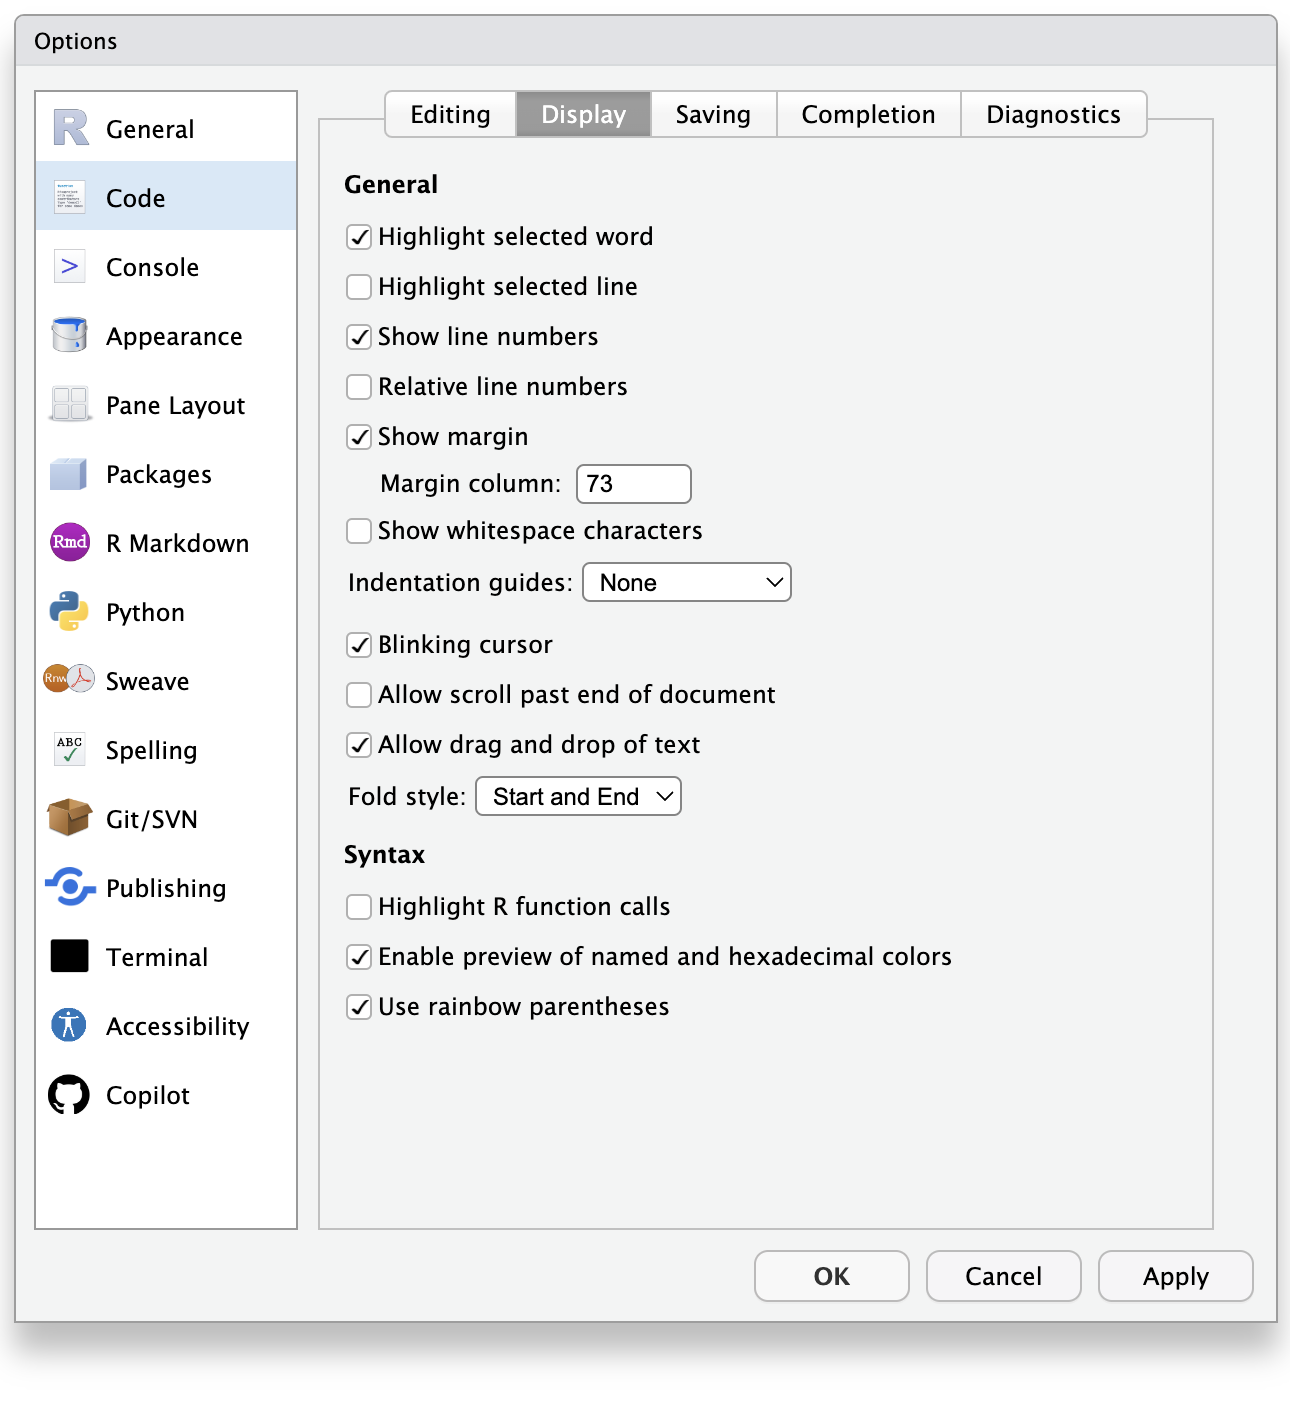
\includegraphics[width=0.8\textwidth,height=\textheight]{fig/temp_show-margin.png}
  \end{center}

  \end{tcolorbox}
\end{enumerate}

\newpage{}

\begin{enumerate}
\def\labelenumi{\arabic{enumi}.}
\setcounter{enumi}{2}
\item
  \href{https://quarto.org/docs/authoring/cross-references.html}{Basics
  of cross-referencing in Quarto} chapters, sections, tables, figures,
  equations, etc.
\item
  \href{https://quarto.org/docs/books/book-crossrefs.html}{How
  cross-referencing works in Quarto Book projects} like this one.

  To reiterate their cautions here\ldots{}

  \begin{tcolorbox}[enhanced jigsaw, coltitle=black, leftrule=.75mm, rightrule=.15mm, breakable, titlerule=0mm, bottomrule=.15mm, left=2mm, colbacktitle=quarto-callout-warning-color!10!white, arc=.35mm, toprule=.15mm, title=\textcolor{quarto-callout-warning-color}{\faExclamationTriangle}\hspace{0.5em}{Reserved prefixes for cross-referencing}, toptitle=1mm, colback=white, bottomtitle=1mm, opacitybacktitle=0.6, opacityback=0, colframe=quarto-callout-warning-color-frame]

  Unless you are creating a cross-reference, avoid using the reserved
  cross-reference prefixes for code cell labels (e.g.~set using the
  \texttt{label} code cell option) and element IDs (set using a
  \texttt{\#} in an attribute).

  The reserved prefixes are: \texttt{fig}, \texttt{tbl}, \texttt{lst},
  \texttt{tip}, \texttt{nte}, \texttt{wrn}, \texttt{imp}, \texttt{cau},
  \texttt{thm}, \texttt{lem}, \texttt{cor}, \texttt{prp}, \texttt{cnj},
  \texttt{def}, \texttt{exm}, \texttt{exr}, \texttt{sol}, \texttt{rem},
  \texttt{eq}, \texttt{sec}.

  You must use the reserved prefixes with their corresponding element
  types (start every figure label with \texttt{fig-}, start every header
  label with \texttt{sec-}, start every table label with \texttt{tbl-},
  and so on).

  Also avoid using underscores (\texttt{\_}) in labels and IDs as this
  can cause problems when rendering to PDF with LaTeX.

  \end{tcolorbox}
\item
  \href{https://quarto.org/docs/authoring/citations.html}{Citations in
  Quarto}
\item
  To follow best practices, we recommend stylizing your code and text
  following the \href{https://style.tidyverse.org}{\textbf{tidyverse}
  style guide}.
\item
  Mathematical expressions in PDF documents require LaTeX formatting
  within inline and display style equations. Rice University provides a
  convenient list of
  \href{https://www.cmor-faculty.rice.edu/~heinken/latex/symbols.pdf}{LaTeX
  mathematical symbols} for your reference.

  \begin{tcolorbox}[enhanced jigsaw, coltitle=black, leftrule=.75mm, rightrule=.15mm, breakable, titlerule=0mm, bottomrule=.15mm, left=2mm, colbacktitle=quarto-callout-note-color!10!white, arc=.35mm, toprule=.15mm, title=\textcolor{quarto-callout-note-color}{\faInfo}\hspace{0.5em}{Note}, toptitle=1mm, colback=white, bottomtitle=1mm, opacitybacktitle=0.6, opacityback=0, colframe=quarto-callout-note-color-frame]

  Letters in math mode are individual variables. If you want to write
  text in math modes such as distribution names, words, etc, then you
  should use LaTeX commands to do so.

  It is best practice to include any distribution names within
  \texttt{\textbackslash{}operatorname\{\}}. For example, we might write
  \(X \sim \operatorname{Normal}(\mu,\, \sigma^2)\).

  When otherwise writing text within an equation, use
  \texttt{\textbackslash{}text\{\}} or
  \texttt{\textbackslash{}textit\{\}} for upright or italic text,
  respectively. For example: \[
  R^2 = 1 - \frac{\text{SSE}}{\text{SST}}.
  \]

  Finally, to get parentheses and brackets to match the size of their
  contents, make use of the \texttt{\textbackslash{}left} and
  \texttt{\textbackslash{}right} commands. Compare the two following
  examples

  \begin{enumerate}
  \def\labelenumii{\arabic{enumii}.}
  \item
    Without \texttt{\textbackslash{}left} and
    \texttt{\textbackslash{}right} \[
    f(x) = \frac{1}{\sqrt{2 \pi \sigma^2}} 
        \exp [-\frac{1}{2} (\frac{x - \mu}{\sigma})^2] 
    \]
  \item
    With \texttt{\textbackslash{}left} and
    \texttt{\textbackslash{}right} \[
    f(x) = \frac{1}{\sqrt{2 \pi \sigma^2}} 
        \exp \left[-\frac{1}{2} \left(\frac{x - \mu}{\sigma}\right)^2 \right] 
    \]
  \end{enumerate}

  \end{tcolorbox}
\end{enumerate}

See the \href{https://quarto.org/docs/guide/}{Comprehensive Quarto
Guide} for more advanced details. See Chapter~\ref{sec-simple} for some
simple examples.

\bookmarksetup{startatroot}

\chapter{Simple examples}\label{sec-simple}

\section{Figures}\label{figures}

Consider customizing your plot themes per-plot---as we do below to
create Figure~\ref{fig-wnba-ht}---or changing the default
\texttt{ggplot()} theme in your document within your \texttt{setup} code
chunks using \texttt{ggplot2::theme\_set()}.

If \textbf{ggplot2} is loaded, the following code sets the default
\texttt{ggplot()} theme to \texttt{theme\_classic()}.

\begin{Shaded}
\begin{Highlighting}[numbers=left,,]
\FunctionTok{theme\_set}\NormalTok{(}\FunctionTok{theme\_classic}\NormalTok{())}
\end{Highlighting}
\end{Shaded}

\begin{figure}

\centering{

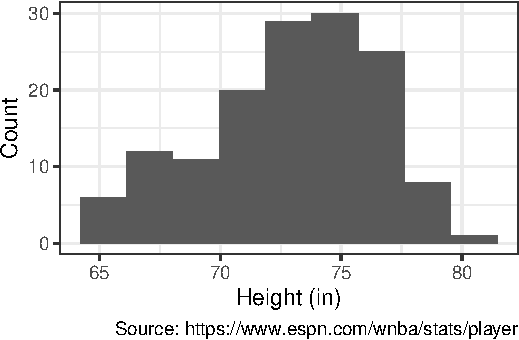
\includegraphics{02-ch2-simple-example_files/figure-pdf/fig-wnba-ht-1.pdf}

}

\caption{\label{fig-wnba-ht}Distribution of heights of WNBA players in
the 2024 season.}

\end{figure}%

\section{Tables}\label{tables}

Your tables should be publication quality. Consider using
\href{https://gt.rstudio.com/articles/gt.html}{\textbf{gt}} (Iannone et
al. 2024) or
\href{https://cran.r-project.org/web/packages/kableExtra/vignettes/awesome_table_in_pdf.pdf}{\textbf{kableExtra}}
(Zhu 2024) to customize your tables. The
\href{https://www.danieldsjoberg.com/gtsummary/}{\textbf{gtsummary}}
package (Sjoberg et al. 2021) may also come in handy.

Table~\ref{tbl-ht-by-pos} shows the average heights of WNBA players by
position.

\begin{longtable}{cr}

\caption{\label{tbl-ht-by-pos}Average WNBA player height by position.}

\tabularnewline

\toprule
Position & Average height (in) \\ 
\midrule
Guard & $70.2$ \\ 
Forward & $74.9$ \\ 
Center & $77.3$ \\ 
\bottomrule

\end{longtable}

\section{\texorpdfstring{Chapter~\ref{sec-simple}
Code}{Chapter~ Code}}\label{sec-simple-code}

The following code was used to create Chapter~\ref{sec-simple}.

\subsection{Code within chapter}\label{code-within-chapter}

\begin{Shaded}
\begin{Highlighting}[numbers=left,,]
\CommentTok{\# Load packages}
\FunctionTok{library}\NormalTok{(tidyverse)}
\FunctionTok{library}\NormalTok{(gt)}

\CommentTok{\# Set default ggplot theme for document}
\FunctionTok{theme\_set}\NormalTok{(}\FunctionTok{theme\_classic}\NormalTok{())}
\CommentTok{\# If using kableExtra tables, print blank cells instead of \textasciigrave{}NA\textasciigrave{}}
\FunctionTok{options}\NormalTok{(}\AttributeTok{knitr.kable.NA =} \StringTok{""}\NormalTok{)}

\CommentTok{\# Load data}
\FunctionTok{load}\NormalTok{(}\StringTok{"data/temp\_wnba.RData"}\NormalTok{)}
\CommentTok{\# Use Freedman{-}Diaconus rule to set binwidth}
\NormalTok{ht\_bw }\OtherTok{\textless{}{-}} \DecValTok{2} \SpecialCharTok{*} \FunctionTok{IQR}\NormalTok{(wnba}\SpecialCharTok{$}\NormalTok{height) }\SpecialCharTok{/} \FunctionTok{nrow}\NormalTok{(wnba)}\SpecialCharTok{\^{}}\NormalTok{(}\DecValTok{1}\SpecialCharTok{/}\DecValTok{3}\NormalTok{)}

\CommentTok{\# Create histogram of height faceted by player position}
\FunctionTok{ggplot}\NormalTok{(wnba, }\FunctionTok{aes}\NormalTok{(height)) }\SpecialCharTok{+}
  \FunctionTok{geom\_histogram}\NormalTok{(}\AttributeTok{binwidth =}\NormalTok{ ht\_bw) }\SpecialCharTok{+}
  \FunctionTok{labs}\NormalTok{(}\AttributeTok{x =} \StringTok{"Height (in)"}\NormalTok{,}
       \AttributeTok{y =} \StringTok{"Count"}\NormalTok{,}
       \AttributeTok{caption =} \StringTok{"Source: https://www.espn.com/wnba/stats/player"}\NormalTok{) }\SpecialCharTok{+}
  \FunctionTok{theme\_bw}\NormalTok{()}
\NormalTok{wnba }\SpecialCharTok{|\textgreater{}} 
  \FunctionTok{group\_by}\NormalTok{(position) }\SpecialCharTok{|\textgreater{}} 
  \FunctionTok{summarize}\NormalTok{(}\AttributeTok{mean\_ht =} \FunctionTok{mean}\NormalTok{(height)) }\SpecialCharTok{|\textgreater{}} 
  \FunctionTok{gt}\NormalTok{() }\SpecialCharTok{|\textgreater{}} 
  \FunctionTok{cols\_label}\NormalTok{(}
    \AttributeTok{position =} \StringTok{"Position"}\NormalTok{,}
    \AttributeTok{mean\_ht =} \StringTok{"Average height (in)"}
\NormalTok{  ) }\SpecialCharTok{|\textgreater{}} 
  \FunctionTok{fmt\_number}\NormalTok{(}\AttributeTok{decimals =} \DecValTok{1}\NormalTok{)}
\CommentTok{\# =======================================================================}
\CommentTok{\# Sample R script for thesis template}
\CommentTok{\#}
\CommentTok{\# Cleans temp\_raw\_wnba.csv dataset, which contains data pulled from}
\CommentTok{\# https://www.espn.com/wnba/stats/player on 2024/06/19}
\CommentTok{\#}
\CommentTok{\# Last updated: 2024/06/19}
\CommentTok{\# =======================================================================}
\FunctionTok{library}\NormalTok{(tidyverse)}

\NormalTok{wnba }\OtherTok{\textless{}{-}} \FunctionTok{read\_csv}\NormalTok{(}\StringTok{"data/temp\_raw\_wnba.csv"}\NormalTok{) }\SpecialCharTok{|\textgreater{}} 
\NormalTok{  janitor}\SpecialCharTok{::}\FunctionTok{clean\_names}\NormalTok{() }\SpecialCharTok{|\textgreater{}} 
  \CommentTok{\# Pull jersey numbers off of names and }
  \CommentTok{\# turn height text into msmt (6\textquotesingle{}4" = 6.3333)}
  \FunctionTok{mutate}\NormalTok{(}\AttributeTok{jersey =} \FunctionTok{str\_extract}\NormalTok{(name, }\StringTok{"[0{-}9]+$"}\NormalTok{),}
         \AttributeTok{name =} \FunctionTok{str\_remove}\NormalTok{(name, }\StringTok{"[0{-}9]+$"}\NormalTok{),}
         \AttributeTok{ht\_ft =} \FunctionTok{parse\_number}\NormalTok{(}\FunctionTok{str\_extract}\NormalTok{(ht, }\StringTok{"\^{}[0{-}9]"}\NormalTok{)),}
         \AttributeTok{ht\_in =} \FunctionTok{parse\_number}\NormalTok{(}\FunctionTok{str\_extract}\NormalTok{(ht, }\StringTok{\textquotesingle{}[0{-}9]+}\SpecialCharTok{\textbackslash{}\textbackslash{}}\StringTok{"$\textquotesingle{}}\NormalTok{)),}
         \AttributeTok{height =}\NormalTok{ ht\_ft }\SpecialCharTok{*} \DecValTok{12} \SpecialCharTok{+}\NormalTok{ ht\_in,}
         \AttributeTok{weight =} \FunctionTok{parse\_number}\NormalTok{(wt),}
         \AttributeTok{position =} \FunctionTok{factor}\NormalTok{(pos,}
                           \AttributeTok{levels =} \FunctionTok{c}\NormalTok{(}\StringTok{"G"}\NormalTok{, }\StringTok{"F"}\NormalTok{, }\StringTok{"C"}\NormalTok{),}
                           \AttributeTok{labels =} \FunctionTok{c}\NormalTok{(}\StringTok{"Guard"}\NormalTok{, }\StringTok{"Forward"}\NormalTok{, }\StringTok{"Center"}\NormalTok{))) }\SpecialCharTok{|\textgreater{}} 
  \FunctionTok{select}\NormalTok{(}\SpecialCharTok{{-}}\FunctionTok{c}\NormalTok{(ht, wt, ht\_ft, ht\_in, pos))}
  
\FunctionTok{save}\NormalTok{(wnba, }\AttributeTok{file =} \StringTok{"data/temp\_wnba.RData"}\NormalTok{)}
\end{Highlighting}
\end{Shaded}

\subsection{Code sourced from external
scripts}\label{code-sourced-from-external-scripts}

\begin{Shaded}
\begin{Highlighting}[numbers=left,,]
\CommentTok{\# =======================================================================}
\CommentTok{\# Sample R script for thesis template}
\CommentTok{\#}
\CommentTok{\# Cleans temp\_raw\_wnba.csv dataset, which contains data pulled from}
\CommentTok{\# https://www.espn.com/wnba/stats/player on 2024/06/19}
\CommentTok{\#}
\CommentTok{\# Last updated: 2024/06/19}
\CommentTok{\# =======================================================================}
\FunctionTok{library}\NormalTok{(tidyverse)}

\NormalTok{wnba }\OtherTok{\textless{}{-}} \FunctionTok{read\_csv}\NormalTok{(}\StringTok{"data/temp\_raw\_wnba.csv"}\NormalTok{) }\SpecialCharTok{|\textgreater{}} 
\NormalTok{  janitor}\SpecialCharTok{::}\FunctionTok{clean\_names}\NormalTok{() }\SpecialCharTok{|\textgreater{}} 
  \CommentTok{\# Pull jersey numbers off of names and }
  \CommentTok{\# turn height text into msmt (6\textquotesingle{}4" = 6.3333)}
  \FunctionTok{mutate}\NormalTok{(}\AttributeTok{jersey =} \FunctionTok{str\_extract}\NormalTok{(name, }\StringTok{"[0{-}9]+$"}\NormalTok{),}
         \AttributeTok{name =} \FunctionTok{str\_remove}\NormalTok{(name, }\StringTok{"[0{-}9]+$"}\NormalTok{),}
         \AttributeTok{ht\_ft =} \FunctionTok{parse\_number}\NormalTok{(}\FunctionTok{str\_extract}\NormalTok{(ht, }\StringTok{"\^{}[0{-}9]"}\NormalTok{)),}
         \AttributeTok{ht\_in =} \FunctionTok{parse\_number}\NormalTok{(}\FunctionTok{str\_extract}\NormalTok{(ht, }\StringTok{\textquotesingle{}[0{-}9]+}\SpecialCharTok{\textbackslash{}\textbackslash{}}\StringTok{"$\textquotesingle{}}\NormalTok{)),}
         \AttributeTok{height =}\NormalTok{ ht\_ft }\SpecialCharTok{*} \DecValTok{12} \SpecialCharTok{+}\NormalTok{ ht\_in,}
         \AttributeTok{weight =} \FunctionTok{parse\_number}\NormalTok{(wt),}
         \AttributeTok{position =} \FunctionTok{factor}\NormalTok{(pos,}
                           \AttributeTok{levels =} \FunctionTok{c}\NormalTok{(}\StringTok{"G"}\NormalTok{, }\StringTok{"F"}\NormalTok{, }\StringTok{"C"}\NormalTok{),}
                           \AttributeTok{labels =} \FunctionTok{c}\NormalTok{(}\StringTok{"Guard"}\NormalTok{, }\StringTok{"Forward"}\NormalTok{, }\StringTok{"Center"}\NormalTok{))) }\SpecialCharTok{|\textgreater{}} 
  \FunctionTok{select}\NormalTok{(}\SpecialCharTok{{-}}\FunctionTok{c}\NormalTok{(ht, wt, ht\_ft, ht\_in, pos))}
  
\FunctionTok{save}\NormalTok{(wnba, }\AttributeTok{file =} \StringTok{"data/temp\_wnba.RData"}\NormalTok{)}
\end{Highlighting}
\end{Shaded}

\bookmarksetup{startatroot}

\chapter*{References}\label{references}
\addcontentsline{toc}{chapter}{References}

\markboth{References}{References}

\phantomsection\label{refs}
\begin{CSLReferences}{1}{0}
\bibitem[\citeproctext]{ref-gt}
Iannone, R., Cheng, J., Schloerke, B., Hughes, E., Lauer, A., Seo, J.,
Brevoort, K., and Roy, O. (2024),
\emph{\href{https://gt.rstudio.com}{Gt: Easily create presentation-ready
display tables}}.

\bibitem[\citeproctext]{ref-gtsummary}
Sjoberg, D. D., Whiting, K., Curry, M., Lavery, J. A., and Larmarange,
J. (2021), {``Reproducible summary tables with the gtsummary package,''}
\emph{{The R Journal}}, 13, 570--580.
\url{https://doi.org/10.32614/RJ-2021-053}.

\bibitem[\citeproctext]{ref-renv}
Ushey, K., and Wickham, H. (2024),
\emph{\href{https://rstudio.github.io/renv/}{Renv: Project
environments}}.

\bibitem[\citeproctext]{ref-kableExtra}
Zhu, H. (2024),
\emph{\href{https://CRAN.R-project.org/package=kableExtra}{kableExtra:
Construct complex table with 'kable' and pipe syntax}}.

\end{CSLReferences}

\cleardoublepage
\phantomsection
\addcontentsline{toc}{part}{Appendices}
\appendix

\chapter{Code availability}\label{sec-code}

This thesis is written using Quarto with \textbf{renv} (Ushey and
Wickham 2024) to create a reproducible environment. All materials
(including the data sets and source files) required to reproduce this
document can be found at the Github repository
\href{https://github.com/github-username/thesis-repo-name}{github.com/GITHUB-USERNAME/THESIS-REPO-NAME}.

This work is licensed under a
\href{http://creativecommons.org/licenses/by-nc-sa/4.0/}{Creative
Commons Attribution-NonCommercial-ShareAlike 4.0 International License}.

\begin{Shaded}
\begin{Highlighting}[numbers=left,,]
\CommentTok{\# =======================================================================}
\CommentTok{\# Sample R script for thesis template}
\CommentTok{\#}
\CommentTok{\# Cleans temp\_raw\_wnba.csv dataset, which contains data pulled from}
\CommentTok{\# https://www.espn.com/wnba/stats/player on 2024/06/19}
\CommentTok{\#}
\CommentTok{\# Last updated: 2024/06/19}
\CommentTok{\# =======================================================================}
\FunctionTok{library}\NormalTok{(tidyverse)}

\NormalTok{wnba }\OtherTok{\textless{}{-}} \FunctionTok{read\_csv}\NormalTok{(}\StringTok{"data/temp\_raw\_wnba.csv"}\NormalTok{) }\SpecialCharTok{|\textgreater{}} 
\NormalTok{  janitor}\SpecialCharTok{::}\FunctionTok{clean\_names}\NormalTok{() }\SpecialCharTok{|\textgreater{}} 
  \CommentTok{\# Pull jersey numbers off of names and }
  \CommentTok{\# turn height text into msmt (6\textquotesingle{}4" = 6.3333)}
  \FunctionTok{mutate}\NormalTok{(}\AttributeTok{jersey =} \FunctionTok{str\_extract}\NormalTok{(name, }\StringTok{"[0{-}9]+$"}\NormalTok{),}
         \AttributeTok{name =} \FunctionTok{str\_remove}\NormalTok{(name, }\StringTok{"[0{-}9]+$"}\NormalTok{),}
         \AttributeTok{ht\_ft =} \FunctionTok{parse\_number}\NormalTok{(}\FunctionTok{str\_extract}\NormalTok{(ht, }\StringTok{"\^{}[0{-}9]"}\NormalTok{)),}
         \AttributeTok{ht\_in =} \FunctionTok{parse\_number}\NormalTok{(}\FunctionTok{str\_extract}\NormalTok{(ht, }\StringTok{\textquotesingle{}[0{-}9]+}\SpecialCharTok{\textbackslash{}\textbackslash{}}\StringTok{"$\textquotesingle{}}\NormalTok{)),}
         \AttributeTok{height =}\NormalTok{ ht\_ft }\SpecialCharTok{*} \DecValTok{12} \SpecialCharTok{+}\NormalTok{ ht\_in,}
         \AttributeTok{weight =} \FunctionTok{parse\_number}\NormalTok{(wt),}
         \AttributeTok{position =} \FunctionTok{factor}\NormalTok{(pos,}
                           \AttributeTok{levels =} \FunctionTok{c}\NormalTok{(}\StringTok{"G"}\NormalTok{, }\StringTok{"F"}\NormalTok{, }\StringTok{"C"}\NormalTok{),}
                           \AttributeTok{labels =} \FunctionTok{c}\NormalTok{(}\StringTok{"Guard"}\NormalTok{, }\StringTok{"Forward"}\NormalTok{, }\StringTok{"Center"}\NormalTok{))) }\SpecialCharTok{|\textgreater{}} 
  \FunctionTok{select}\NormalTok{(}\SpecialCharTok{{-}}\FunctionTok{c}\NormalTok{(ht, wt, ht\_ft, ht\_in, pos))}
  
\FunctionTok{save}\NormalTok{(wnba, }\AttributeTok{file =} \StringTok{"data/temp\_wnba.RData"}\NormalTok{)}
\end{Highlighting}
\end{Shaded}

\begin{Shaded}
\begin{Highlighting}[numbers=left,,]
\CommentTok{\# =======================================================================}
\CommentTok{\# Sample R script for thesis template}
\CommentTok{\#}
\CommentTok{\# Doesn\textquotesingle{}t do anything useful}
\CommentTok{\#}
\CommentTok{\# Last updated: 2024/08/24}
\CommentTok{\# =======================================================================}

\FunctionTok{print}\NormalTok{(}\StringTok{"Hello, Amherst!"}\NormalTok{)}
\end{Highlighting}
\end{Shaded}

\chapter{Corrections}\label{sec-corrections}

This section may be excluded if no corrections are made to your thesis
after initial submission to the department and before final submission
to the college.

Per the
\href{https://www.amherst.edu/academiclife/departments/mathematics-statistics/major-in-statistics/honors-in-statistics/thesis-regulations}{Statistics
Honors Thesis Regulations}:

\begin{quote}
Corrections to theses may be made after the date on which they are due
in the Department's hands. Corrections may be made to the body of the
thesis, but every such correction will be acknowledged in a list under
the heading ``Corrections,'' along with the statement ``When originally
submitted, this honors thesis contained some errors which have been
corrected in the current version. Here is a list of the errors that were
corrected.'' This list will be given on a sheet or sheets to be appended
to the thesis. Corrections to spelling, grammar, or typography may be
acknowledged by a general statement such as ``30 spellings were
corrected in various places in the thesis, and the notation for definite
integral was changed in approximately 10 places.'' However, any
correction that affects the meaning of a sentence or paragraph should be
described in careful detail, and substantial additions to the thesis
will not be allowed. Questions about what should appear in the
``Corrections'' should be directed to the Chair. Electronic versions of
the thesis, technical appendix, and necessary data and supplemental
files must all be updated at the time of correction as well.
\end{quote}

When originally submitted, this honors thesis contained some errors
which have been corrected in the current version. Here is a list of the
errors that were corrected.

\begin{enumerate}
\def\labelenumi{\arabic{enumi}.}
\tightlist
\item
  \ldots{}
\item
  \ldots{}
\end{enumerate}




\end{document}
